\chapter{AST PDF Generator}
\label{Tutorial:chapter_AST_PDF_Generator}

\paragraph{What To Learn From This Example}
This example demonstrates a mechanism for generating a visualization
of the AST using pdf files.  A pdf file is generated and can be viewed 
using {\tt acroread}.  The format is suitable for much larger input 
programs than the example shown in previous chapters using dot
format~\ref{Tutorial:chapterASTWholeGraphGenerator}.
This mechanism can support the visualization of input files around 100K 
lines of code.

\begin{figure}[!h]
{\indent
{\mySmallFontSize


% Do this when processing latex to generate non-html (not using latex2html)
\begin{latexonly}
   \lstinputlisting{\TutorialExampleDirectory/AST_PDF_Generator.C}
\end{latexonly}

% Do this when processing latex to build html (using latex2html)
\begin{htmlonly}
   \verbatiminput{\TutorialExampleDirectory/AST_PDF_Generator.C}
\end{htmlonly}

% end of scope in font size
}
% End of scope in indentation
}
\caption{Example source code to read an input program and generate a PDF file to represent the AST.}
\label{Tutorial:exampleAST_PDF_Generator}
\end{figure}

\begin{figure}[!h]
{\indent
{\mySmallFontSize


% Do this when processing latex to generate non-html (not using latex2html)
\begin{latexonly}
   \lstinputlisting{\TutorialExampleDirectory/inputCode_ASTGraphGenerator.C}
\end{latexonly}

% Do this when processing latex to build html (using latex2html)
\begin{htmlonly}
   \verbatiminput{\TutorialExampleDirectory/inputCode_ASTGraphGenerator.C}
\end{htmlonly}

% end of scope in font size
}
% End of scope in indentation
}
\caption{Example source code used as input to generate the PDF file of the AST.}
\label{Tutorial:exampleInputCode_AST_PDF_Generator}
\end{figure}

\begin{figure}
%\centerline{\epsfig{file=\TranslatorExampleDirectory/AST-pdf2.ps,height=0.75\linewidth,width=1.0\linewidth,angle=0}}
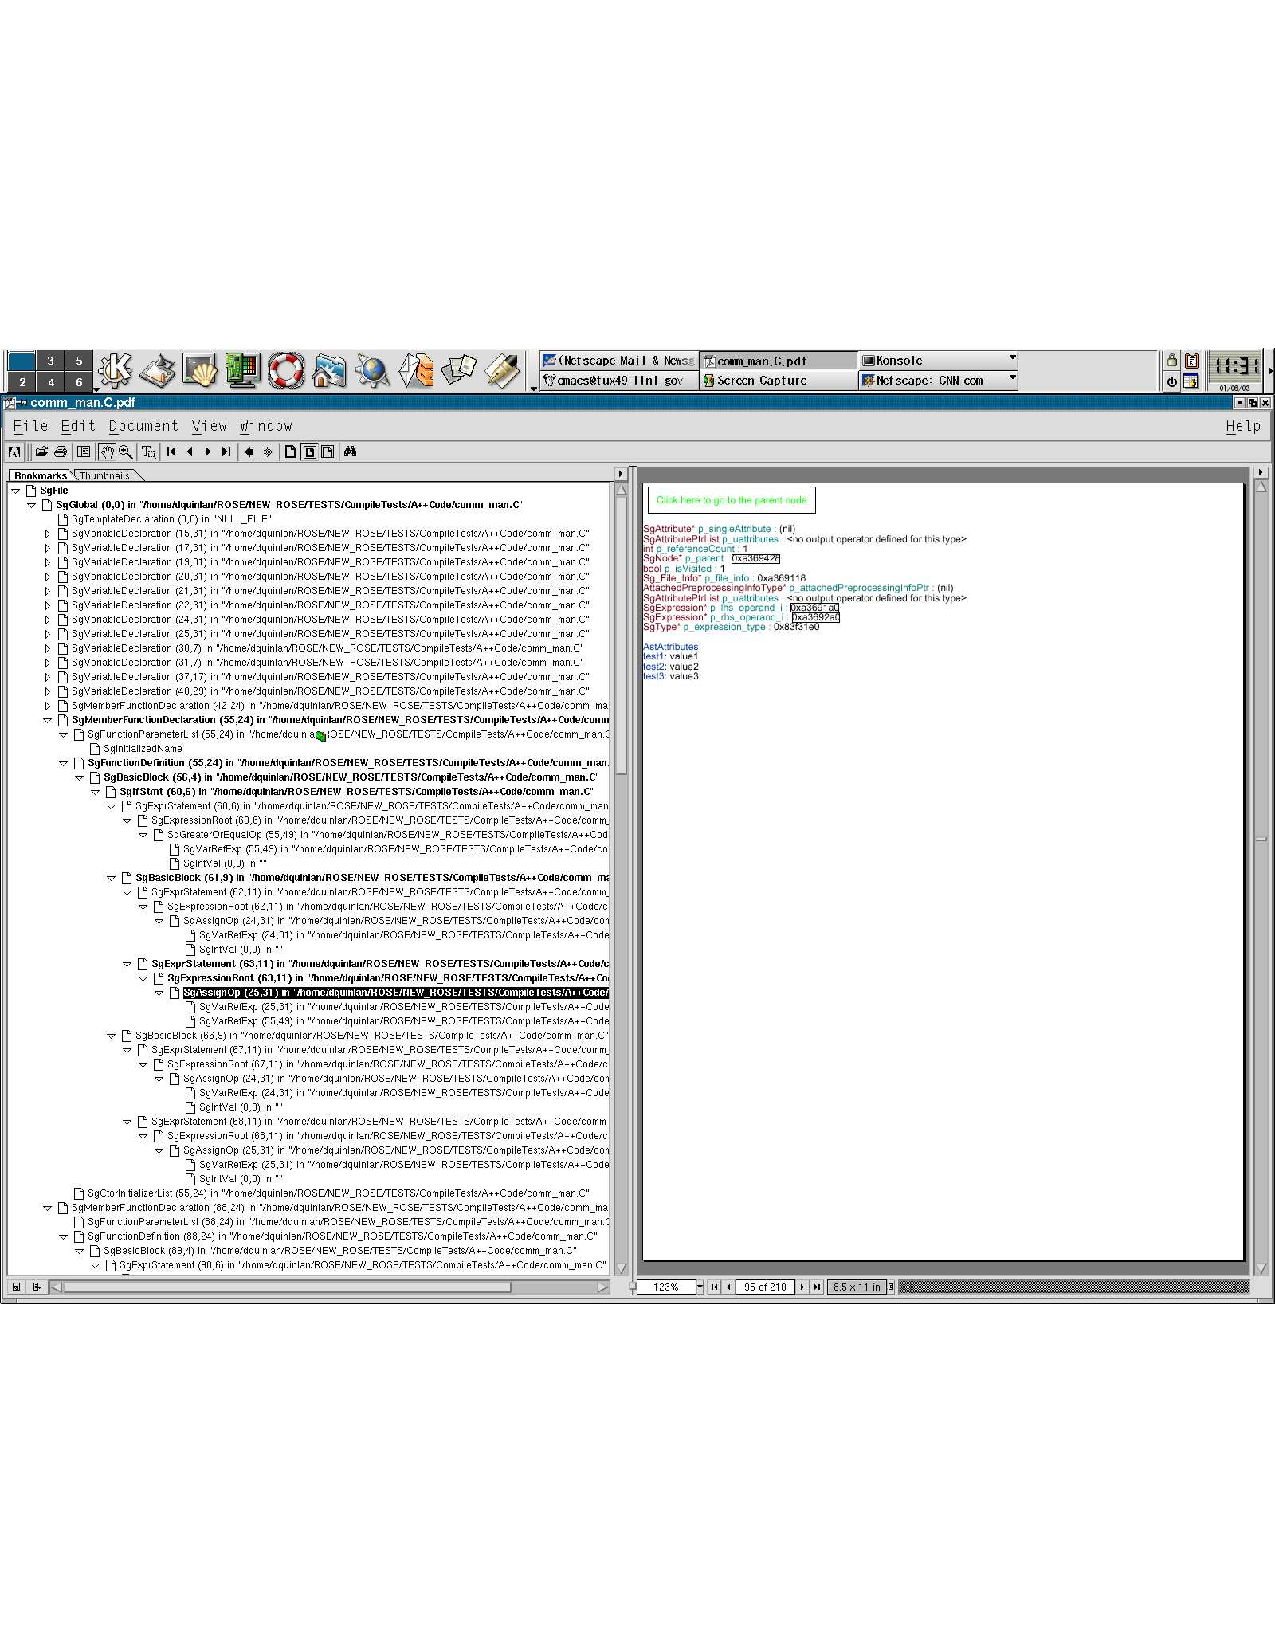
\includegraphics[angle=90,scale=0.85]{\TranslatorExampleDirectory/AST-pdf2}
\caption{Example output from translator which outputs PDF representation of AST. The
    generated PDF file makes use of the bookmark mechanism to expand and collapse 
    parts of the AST.}
\label{tutorial:exampleOutputCodePDF}
\end{figure}

The program in figure~\ref{Tutorial:exampleAST_PDF_Generator} calls 
an internal ROSE function that traverses the AST and generates 
an ASCI file in {\tt dot} format.
Figure~\ref{Tutorial:exampleInputCode_ASTGraphGenerator} shows an input
code which is processed to generate a graph of the AST, generating a 
{\tt pdf} file.   The {\tt pdf} file is then processed
using {\tt acroread} to generate a GUI for viewing the AST.

A standalone utility tool, called \textit{pdfGenerator} is provided within
ROSE. It is available from
\textit{ROSE\_BUILD/exampleTranslators/PDFGenerator} or
\textit{ROSE\_INS/bin}. Users can use it to generate AST in a pdf format
from an input code.

   Figure~\ref{tutorial:exampleOutputCodePDF} displays on the left hand side the individual
C++ nodes in ROSE's intermediate representation (IR).  The page on the right hand side
shows that IR nodes member data. Pointers in boxes can be clicked on to navigate the AST
(or nodes in the tree hierarchy can be clicked on jump to any location in the AST.
This representation shows only the IR nodes that are traversed by the standard traversal
(no SgSymbol or SgType IR nodes are presented in this view of the AST).

% Alternative description
The output of this translator is shown in figure \ref{tutorial:exampleOutputCodePDF}.  The left hand side
of the screen is a tree with click-able nodes to expand/collapse the subtrees.
The right hand side of the screen is a description of the data at a particular 
node in the AST (the node where the user has clicked the left mouse button).
This relatively simple view of the AST is useful for debugging transformation and finding
information in the AST required by specific sorts of analysis.  It is also useful
for developing an intuitive feel for what information is in the AST, how it is organized, 
and where it is stored.

